% C037 独立新增图：a=3, c=5, b=4 的顶点/焦点数轴。
% 说明：这是一张新增图，不替换、不覆盖任何原有 TikZ 文件。
\begin{center}
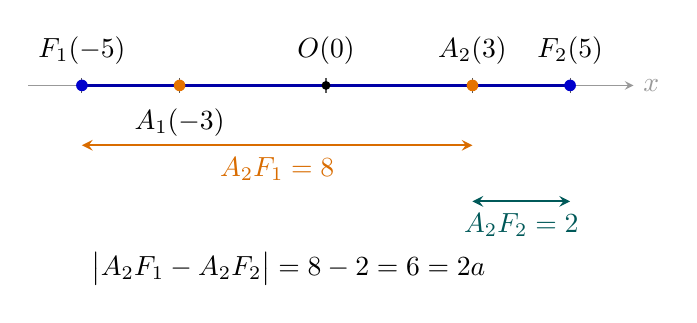
\begin{tikzpicture}[x=0.62cm,y=0.95cm,>=stealth]
  \draw[->, gray!80] (-6.1,0)--(6.3,0) node[right] {$x$};
  \draw[line width=1.1pt,blue!65!black] (-5,0)--(5,0);
  \foreach \x in {-5,-3,0,3,5} {
    \draw[black!65] (\x,0.10)--(\x,-0.10);
  }
  \fill[blue!80!black] (-5,0) circle (2.1pt);
  \fill[blue!80!black] (5,0) circle (2.1pt);
  \fill[orange!90!black] (-3,0) circle (2.1pt);
  \fill[orange!90!black] (3,0) circle (2.1pt);
  \fill[black] (0,0) circle (1.6pt);
  \node[above=4pt] at (-5,0) {$F_1(-5)$};
  \node[below=5pt] at (-3,0) {$A_1(-3)$};
  \node[above=4pt] at (0,0) {$O(0)$};
  \node[above=4pt] at (3,0) {$A_2(3)$};
  \node[above=4pt] at (5,0) {$F_2(5)$};
  \draw[<->,line width=.7pt,orange!85!black] (-5,-0.8)--(3,-0.8)
    node[midway,below=3pt,fill=white,inner sep=1pt] {$A_2F_1=8$};
  \draw[<->,line width=.7pt,teal!70!black] (3,-1.55)--(5,-1.55)
    node[midway,below=3pt,fill=white,inner sep=1pt] {$A_2F_2=2$};
  \node[anchor=west] at (-5,-2.45)
    {$\bigl|A_2F_1-A_2F_2\bigr|=8-2=6=2a$};
\end{tikzpicture}
\end{center}
